\documentclass[12pt,english]{article}
\usepackage[T1]{fontenc}
\usepackage[latin9]{inputenc}
\usepackage{geometry}
\geometry{verbose,tmargin=1in,bmargin=0.9in,lmargin=0.9in,rmargin=1in,headheight=1cm,headsep=1cm,footskip=1cm}
\usepackage{amstext}
\usepackage{amssymb}
\usepackage{amsthm}
\usepackage{babel}
\usepackage{array}
\usepackage{color}
\usepackage{amsmath}
\usepackage{graphicx}
\usepackage{adjustbox}
\usepackage{color}
\usepackage{subfig}
%\usepackage{epstopdf,epsfig}
\usepackage{float}	
\usepackage{color}
\usepackage{booktabs,caption}
\usepackage{threeparttable}
% \usepackage{hyperref}
\usepackage{tgpagella} % delete this to change back to the default font
\usepackage[toc]{appendix}
\usepackage[numbers]{natbib}
%\bibliographystyle{abbrvnat}
\setcitestyle{authoryear,open={(},close={)}}
\definecolor{newred}{RGB}{144,23,23}
\usepackage{rotating}
\usepackage[outdir=./]{epstopdf,epsfig}
\usepackage{csvsimple}
\bibliographystyle{abbrvnat}
%\tolerance=1000
%\usepackage[framed,numbered,autolinebreaks,useliterate]{mcode}
\usepackage{appendix}
\usepackage{threeparttable}
\theoremstyle{remark}
\newtheorem{remark}{Remark}
\newtheorem{definition}{Definition}
\newtheorem{proposition}{Proposition}
\newtheorem{assumption}{Assumption}
\newtheorem{fact}{Fact}
%\newtheorem{prop}{Proposition}[section]
%\usepackage{threeparttable}

\newcommand{\sym}[1]{\rlap{#1}}
\newcommand{\Mc}{M{\large\raisebox{0.35ex}{{{\smash{c}}}}}}
\newcommand{\E}{\mathbb{E}}


\usepackage{setspace}
\onehalfspacing

\usepackage[unicode=true,
bookmarks=true,bookmarksnumbered=false,bookmarksopen=false,pdfborder={0 0 0},backref=false,colorlinks=true]
{hyperref} 
% breaklinks=true
\hypersetup{pdftitle={IBCA},
	pdfauthor={McMiken},
	linkcolor=red, citecolor=newred, urlcolor=blue, filecolor=blue}

\usepackage{listings}
\lstset{language=Matlab}
\usepackage{tikz}
\usetikzlibrary{arrows}



\providecommand{\keywords}[1]
{
	\small	
	\textbf{\textit{Keywords---}} #1
}

\begin{document}
	\title{PE Investment
	}
	\date{\today} %\today.}
	\author{Shane \Mc Miken}
	
	\maketitle
	\section*{Benchmark PE Firm Investment Model}
	A continuum of mass 1 of ex-ante identical firms solve the following dynamic profit maximization problem, subject to idiosyncratic productivity shocks z:
	\begin{align*}
		V(z,k) &= \max{k'} \bigg[zk^\alpha - p k' + p(1-\delta)k -AC(z,k,k') + \frac{1}{1+r} \E(V(z',k')|z)\bigg]
		\\
		\log z &= \rho \log z_{t-1} + \sigma \epsilon, \epsilon \sim N(0,1)
		\\
		AC(z,k,k') &= \frac{\gamma_c}{2} \bigg(\frac{k' -(1-\delta)k}{k}\bigg)^2 + \gamma_f y \mathbb{I}(k' \neq (1-\delta)k)
	\end{align*}
	I solve the model for the following calibrations:
	\begin{table}[h]
		\begin{center}
			\begin{tabular}{ p{3cm}|p{1cm}|p{1cm}|p{1cm}|p{1cm}|p{1cm}|p{1cm}|p{1cm}|p{1cm}  }
				& $\alpha$  & p & $\delta$ & r & $\rho$ & $\sigma$ & $\gamma_c$ & $\gamma_f$ \\
				\hline
				No AC & 0.7  & 1.2 & 0.1 & 0.04 & 0.8 & 0.2 & 0 & 0 \\
				\hline
				Convex AC & 0.7  & 1.2 & 0.1 & 0.04 & 0.8 & 0.2 & 2.5 & 0 \\
				Fixed AC & 0.7  & 1.2 & 0.1 & 0.04 & 0.8 & 0.2 & 0 & 0.05 \\
			\end{tabular}
		\end{center}
	\end{table}
	\section*{Extracting Results from the Model}
	I solve the model using value function iteration and the Howard acceleration algorithm. I compute the ergodic distribution $\tilde \mu$ using Young's algorithm. The resulting plots come from the model's solution:
	
	\begin{figure}		
		\begin{minipage}{.5\linewidth}
			\centering
			\subfloat[]{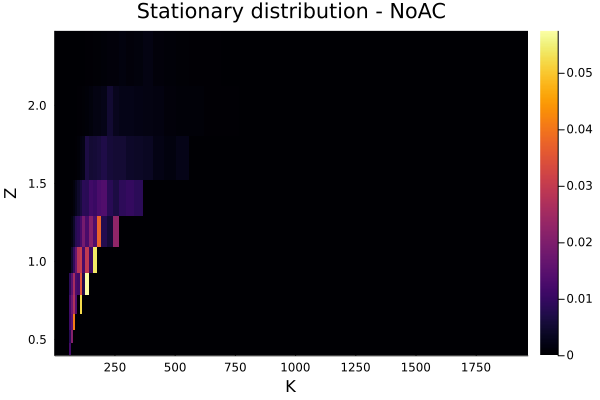
\includegraphics[scale=.4]{stationarydistribution_NoAC.png}}
		\end{minipage}%
		\begin{minipage}{.5\linewidth}
			\centering
			\subfloat[]{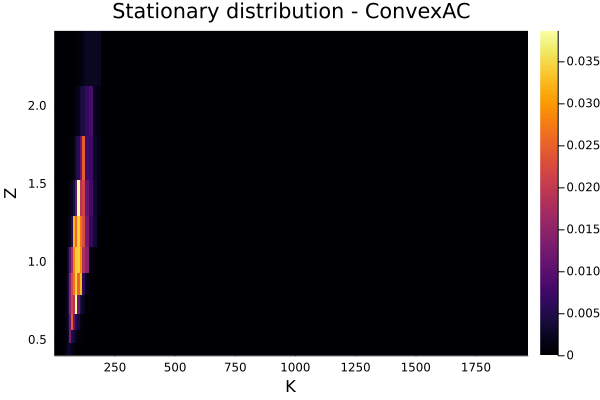
\includegraphics[scale=.4]{stationarydistribution_ConvexAC.png}}
		\end{minipage}\par\medskip
		\centering
		\subfloat[]{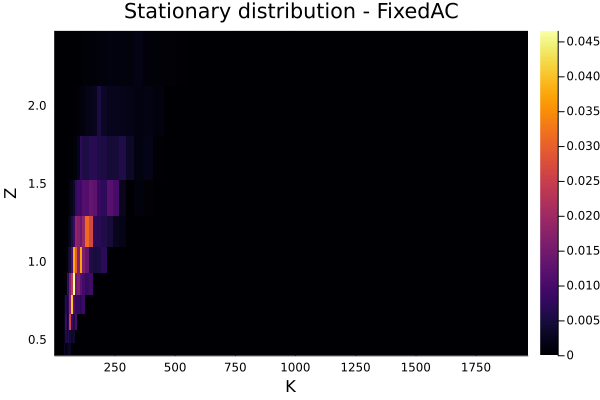
\includegraphics[scale=.4]{stationarydistribution_FixedAC.png}}
		
		\caption{Stationary Distribution $\tilde \mu$ on $\mathcal{Z} \times \mathcal{K}$}
		\label{fig:main}
	\end{figure}

	\begin{figure}
		\begin{minipage}{.5\linewidth}
			\centering
			\subfloat[]{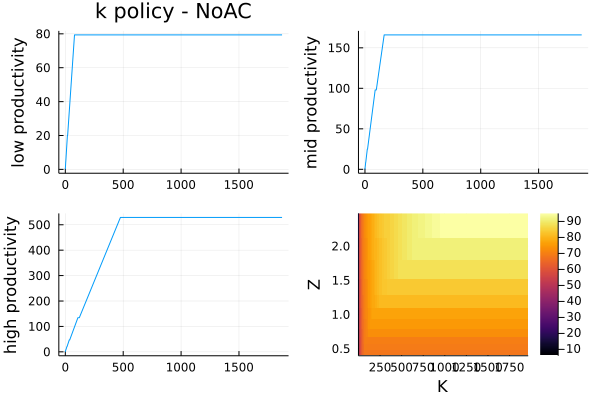
\includegraphics[scale=.4]{policyfunctions_NoAC.png}}
		\end{minipage}%
		\begin{minipage}{.5\linewidth}
			\centering
			\subfloat[]{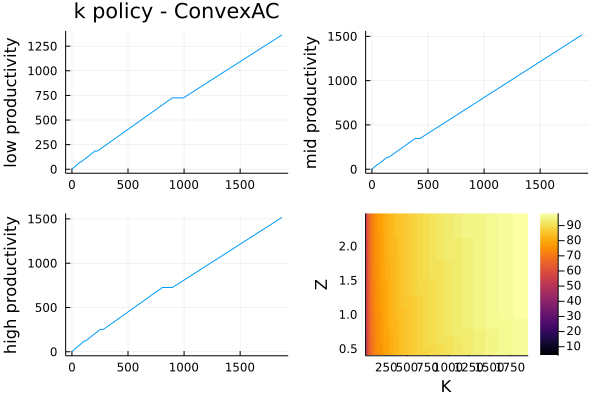
\includegraphics[scale=.4]{policyfunctions_ConvexAC.png}}
		\end{minipage}\par\medskip
		\centering
		\subfloat[]{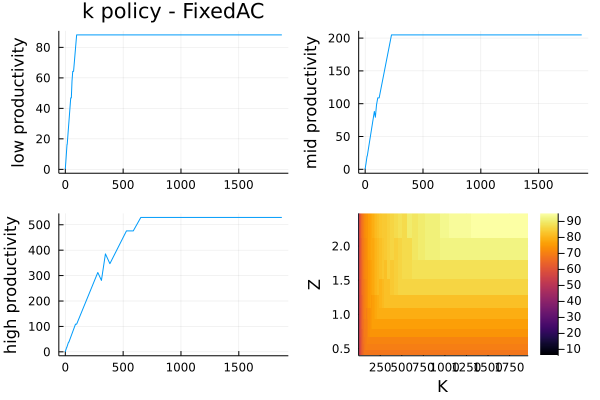
\includegraphics[scale=.4]{policyfunctions_FixedAC.png}}
		
		\caption{Policy functions $k'(z,k)$ on $\mathcal{Z} \times \mathcal{K}$ at three levels 'low productivity' z = 0.61, 'mid productivity' z = 1 and 'high productivity' z = 1.65}
		\label{fig:main}
	\end{figure}

	\begin{figure}
		\begin{minipage}{.5\linewidth}
			\centering
			\subfloat[]{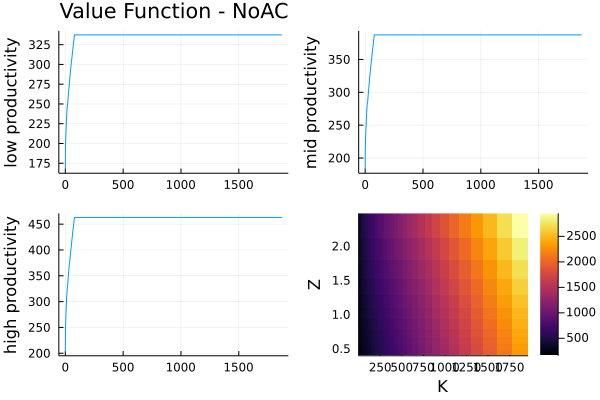
\includegraphics[scale=.4]{valuefunction_NoAC.png}}
		\end{minipage}%
		\begin{minipage}{.5\linewidth}
			\centering
			\subfloat[]{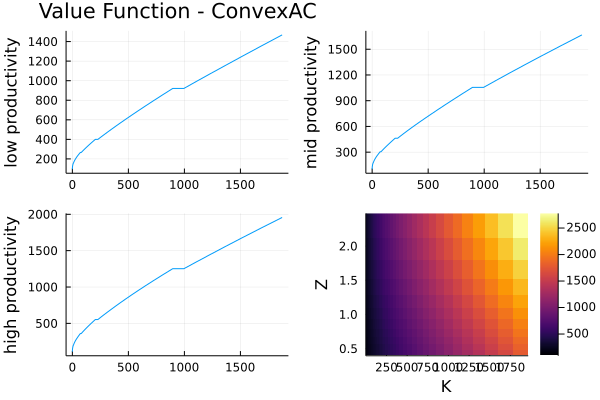
\includegraphics[scale=.4]{valuefunction_ConvexAC.png}}
		\end{minipage}\par\medskip
		\centering
		\subfloat[]{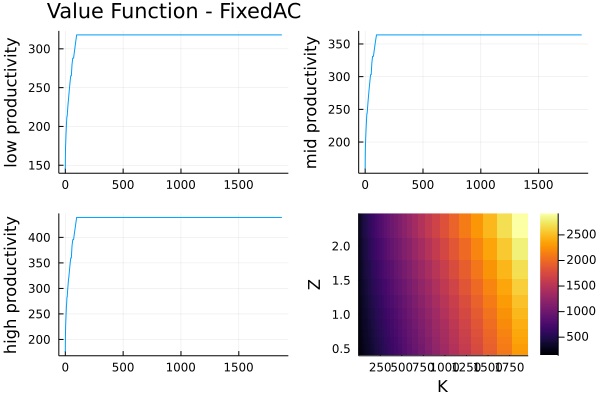
\includegraphics[scale=.4]{valuefunction_FixedAC.png}}
		
		\caption{Value functions $V(z,k,k'(z,k))$ on $\mathcal{Z} \times \mathcal{K}$ at three levels 'low productivity' z = 0.61, 'mid productivity' z = 1 and 'high productivity' z = 1.65}
		\label{fig:main}
	\end{figure}

	\begin{figure}
		\begin{minipage}{.5\linewidth}
			\centering
			\subfloat[]{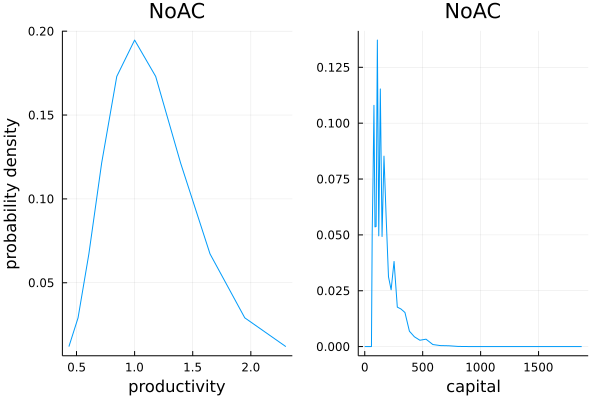
\includegraphics[scale=.4]{marginaldistributions_NoAC.png}}
		\end{minipage}%
		\begin{minipage}{.5\linewidth}
			\centering
			\subfloat[]{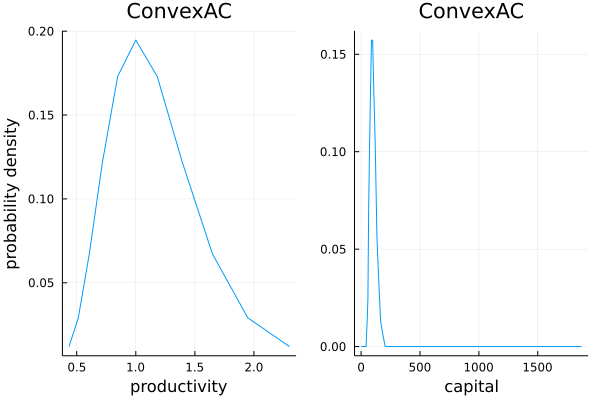
\includegraphics[scale=.4]{marginaldistributions_ConvexAC.png}}
		\end{minipage}\par\medskip
		\centering
		\subfloat[]{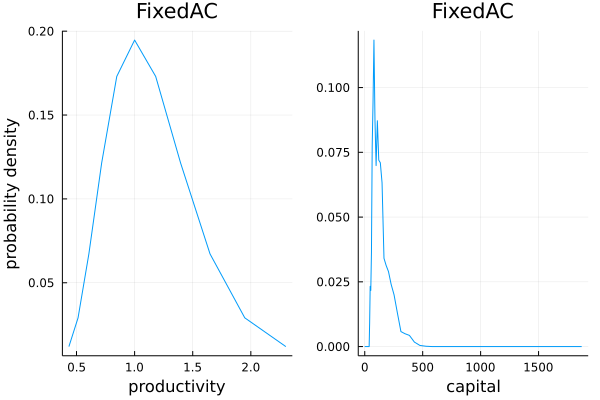
\includegraphics[scale=.4]{marginaldistributions_FixedAC.png}}
		
		\caption{Marginal distributions of capital $k$ and productivity $z$}
		\label{fig:main}
	\end{figure}
	
	\begin{figure}
		\begin{minipage}{.5\linewidth}
			\centering
			\subfloat[]{\label{NoAC}\csvautotabular{correlationmatrix_NoAC.csv}}
		\end{minipage}%
		\begin{minipage}{.5\linewidth}
			\centering
			\subfloat[]{\label{FixedAC}\csvautotabular{correlationmatrix_ConvexAC.csv}}
		\end{minipage}\par\medskip
		\centering
		\subfloat[]{\label{main:ConvexAC}\csvautotabular{correlationmatrix_FixedAC.csv}}
		
		\caption{Moments of $X = [\log k \; \log z \; \log y \; i/k]$ on $\tilde \mu$, the first row is $\E X$ beneath are the correlation matrices. Top left: NoAC, Top right: ConvexAC, Bottom: FixedAC.}
	\end{figure}
	
	\begin{figure}
			\begin{center}
			\begin{tabular}{ | m{2cm} | m{1cm}| m{1cm} | m{1cm} |m{1cm} |m{1cm} |m{1cm} |} 
				\hline
				& $\E_{\mu(y)}$ & $\E_{\mu(i)}$ & $\E_{\mu(k)}$ & $\E_{\mu(V)}$ & $\E_{\mu(z)}$ & $\bar{TFP}$ \\ 
				\hline
				NoAC & 36.17 & 21.23 & 142.06 & 481.66 & 1.06 & 1.13 \\ 
				\hline
				FixedAC & 31.14 & 13.54 & 115.37 & 411.12 & 1.06 & 1.12 \\ 
				\hline
				ConvexAC & 26.65 & 9.8 & 96.03 & 348.66 & 1.06 & 1.09 \\ 
				\hline
			\end{tabular}
		\end{center}
		\caption{Aggregates: implied $\bar{TFP}$ is larger than average of true underlying productivity because more productive/larger firms produce more.}
	\end{figure}
	\clearpage
	\begin{figure}
		\begin{minipage}{.5\linewidth}
			\centering
			\subfloat[]{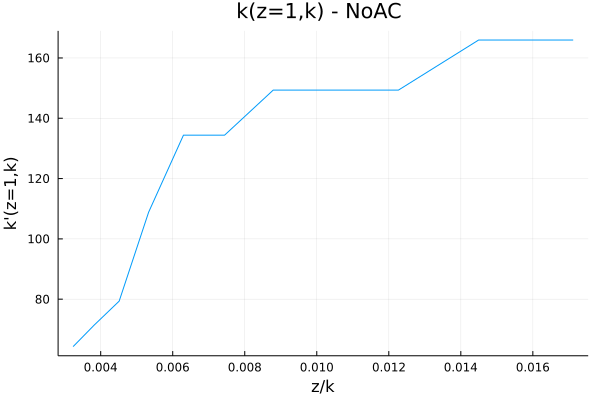
\includegraphics[scale=.4]{eqpolicy_NoAC.png}}
		\end{minipage}%
		\begin{minipage}{.5\linewidth}
			\centering
			\subfloat[]{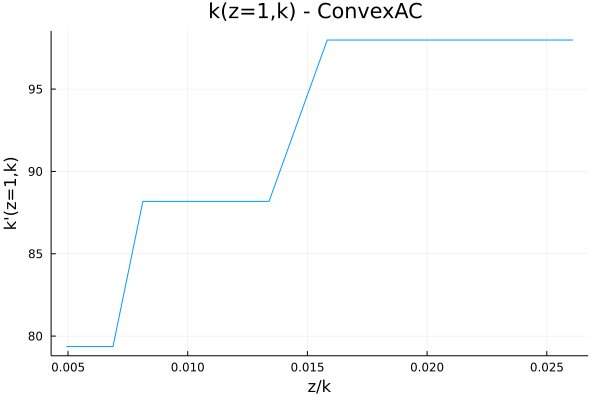
\includegraphics[scale=.4]{eqpolicy_ConvexAC.png}}
		\end{minipage}\par\medskip
		\centering
		\subfloat[]{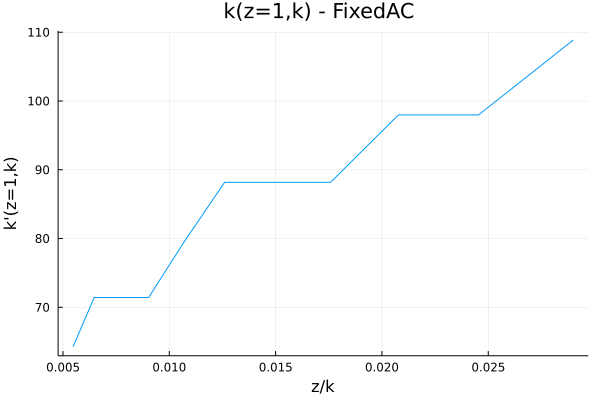
\includegraphics[scale=.4]{eqpolicy_FixedAC.png}}
		
		\caption{$k^*(z,k)$ policy versus $z/k$}
		\label{fig:main}
	\end{figure}
	\paragraph{Policy functions}differ with respect at their inaction regions in $z/k$ and the jumps in $k'$. The calibration with convex adjustment costs features the largest inaction regions along with the largest jumps; since the cost of adjusting is increasing in capital, firms require that $z/k$ increases a lot to induce investment to a much higher target level. Fixed adjustment costs imply there is a cost associated with adjusting capital, hence firms will adjust their capital if the benefit from adjusting is greater than the fixed cost. The inaction regions smaller than those of the convex cost calibration reflecting the target capital need only move a bit to overcome the fixed cost of adjustment. The calibration with no adjustment costs bears resemblance to a convex function. 

\end{document}